\subsubsection{Number Theory, Arithmetic Geometry, Diophantine Equations}
\index{Stoll, Michael}

\paragraph{Research Team}

Michael Stoll (Professor),
Sebastian Stamminger, (PhD Student, thesis defense in December~2005),
Jan Steffen M\"uller (PhD Student, since September~2006)

\medskip

Most of my research studies the set of
rational points on a curve.  In more elementary terms, I~am looking at the set
of solutions in rational numbers to an equation $F(x, y) = 0$, where
$F$ is a polynomial with integer coefficients.

Such curves are classified according to their genus~$g \ge 0$.
The case $g = 0$ is well understood.
Curves with $g = 1$ either have no rational points at all,  or the set of
rational points forms a finitely generated abelian group;
the problem is then to find generators of this group. Curves
with  $g \ge 2$ have only  finitely many rational points; here the
problem is to find all of them.

There are no general methods that are known to solve these problems.
However, there are methods available that solve these problems in
many concrete cases. Part of my  research tries to extend the range
of cases we can deal with. The other part is about proving general
results.


\paragraph{Highlights}

%500 words about highlights in 2006

In this year, I was mostly continuing work on projects that feature in
previous research reports, with the aim of getting papers ready for
publication. For example, the paper~\cite{Stoll2} on the generalized
Fermat Equation $x^2 + y^3 = z^7$ that I wrote with Bjorn Poonen and
Ed~Schaefer has been finished, submitted and accepted for publication.
Another area of ongoing work is the project on `Explicit $n$-descent
on elliptic curves', which is a joint effort with John Cremona, Tom
Fisher, Cathy O'Neil and Denis Simon. We have finished and submitted
the first two of a series of papers describing our
results~\cite{StollandCFOS1,StollandCFOS2}; the first has just been
accepted by the `Journal f\"ur die reine und angewandte Mathematik'.
Two more papers
are in preparation. Finally, a paper which gives an overview over a
computational experiment that I performed with Nils Bruin has just been
recommended for publication in `Experimental Mathematics',
see~\cite{Stoll4}. Three further papers that describe the details of the
algorithms we used are being written or in preparation. Below,
I will give some more detail on this experiment.

The question we were studying is the following. Given a curve of
genus at least~$2$, defined over the field of rational numbers, is it
possible to decide algorithmically whether it has any rational points?
The most obvious first case to look at is when the genus is~$2$.
In this case, the curve has an equation of the form
\[ y^2 = f_6 x^6 + f_5 x^5 + f_4 x^4 + f_3 x^3 + f_2 x^2 + f_1 x + f_0 \]
where the polynomial on the right hand side has degree $5$ or~$6$ and
does not have multiple roots. For these curves, a number of algorithms
is available and implemented (many of them based on research I have
done). To make the computations feasible and on the other hand not
dependent on random choices, we decided to consider {\em all} such
curves with coefficients $f_0, f_1, \dots, f_6$ from $\{-3,-2,1,0,1,2,3\}$.
Identifying `isomorphic' curves, we had to study about 200,000
different curves.

For each of these curves, we first tried to find a rational point.
This was successful for about 140,000 of them. In a next step, we
checked the curves for `local solubility', which is a necessary
condition for rational points to exist. For example, it may be the
case that the equation does not even have solutions in real numbers.
We were able to prove in this way for about 30,000 curves that they
do not possess rational points. Then we applied a `2-cover descent'
to the remaining about 30,000 curves. This allowed us to test a
stronger necessary condition, at the cost of a much more involved
computation. In this way, all but about 1,500 curves were shown to
have no rational points. Finally, for these remaining curves, we used
another method which needs still more computation, and were able to
prove that none of them has a rational point. For 42 curves, we had
to assume a standard conjecture, otherwise our results are
unconditional. So we could answer the question for all our curves.
This is a very nice result and supports the view that it should
always be possible to decide whether rational points exist or not.


%Pictures are to be included via:
%
\begin{figure}[ht]
  \begin{center}
    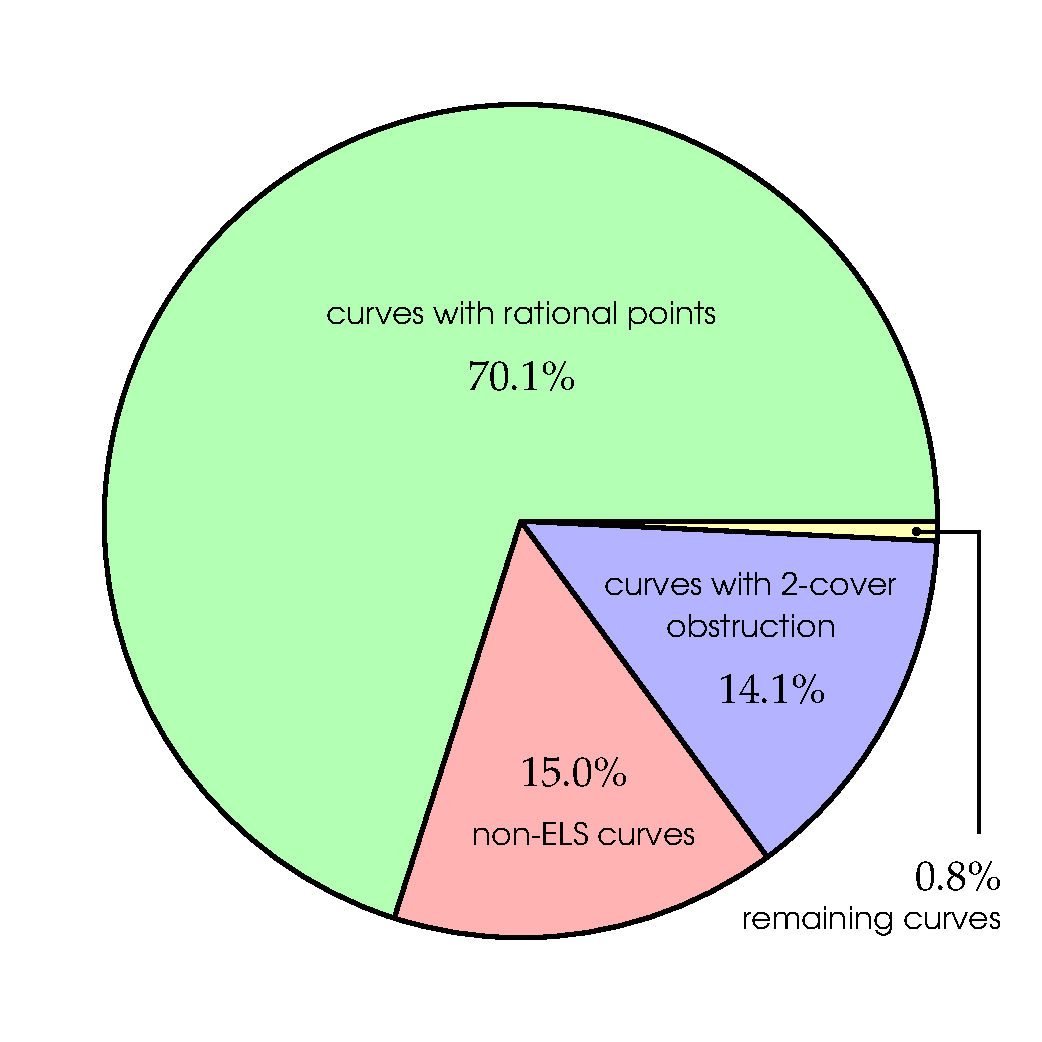
\includegraphics[width=\hsize]{Stoll/profStoll-fig1.pdf}
    \mycaption{Curve statistics (ELS = everywhere locally solvable)}\label{fig:profStoll}
   \end{center}
\end{figure}

\nocite{Stoll1}
\nocite{Stoll3}
\nocite{Stoll5}
\nocite{Stamminger}
\nocite{Stoll6}

\paragraph{Organization}
% list the (research) events you have organized, if any,

\begin{enumerate}
  \item Co-organization of a joint ``Seminar on Algebraic and Arithmetic
        Geometry'' between Universit\"at G\"ottingen, Universit\"at Hannover
        and Jacobs University Bremen
  \item Organization of a training weekend for the German IMO team
        (with Dierk Schleicher and Alexei Belov).
\end{enumerate}

\paragraph{Collaborations}

\begin{enumerate}
  \item {\sl University of California at Berkeley, USA} \\
        Prof.~B.~Poonen \\
        Generalized Fermat Equations, Rational Points on Curves
  \item {\sl University of Santa Clara, California, USA} \\
        Prof.~E.F.~Schaefer \\
        Generalized Fermat Equations
  \item {\sl University of Nottingham, UK} \\
        Prof.~J.E.~Cremona \\
        Descent on Elliptic Curves
  \item {\sl Cambridge, UK} \\
        Dr.~T.A.~Fisher \\
        Descent on Elliptic Curves
  \item {\sl Columbia University, New York, USA} \\
        Asst.~Prof.~C.~O'Neil \\
        Descent on Elliptic Curves
  \item {\sl Universit\'e de Caen, France} \\
        Dr.~D.~Simon \\
        Descent on Elliptic Curves
  \item {\sl Simon Fraser University, Vancouver, Canada} \\
        Asst.~Prof.~N.~Bruin \\
        Rational Points on Curves
  \item {\sl Jacobs University Bremen} \\
        Dr.~S.~Baier \\
        Rational Points on Curves
\end{enumerate}


\paragraph{Grants}
% list the running grants in 2006, if none have been received, please delete this
% subsection.
\begin{enumerate}
  \item Funded by EU, \emph{Galois Theory and Explicit Methods}
        (FP\,6 Research and Training Network, from October~2006;
        I am an external member of the node in Essen)
  \item Funded by DFG, \emph{Arithmetic of K3 Surfaces}

  \item Funded by DFG, \emph{Support for a workshop ``Rational Points on Curves
        and Higher-Dimensional Varieties: Theory  and Explicit Methods''
        at Jacobs University Bremen}, (July 21--28, 2007)
\end{enumerate}


%\paragraph{Awards, Prizes}
% list the grants you have received in 2006, if none have been received, please delete this
% subsection.
%\begin{enumerate}
%\item
%\item
%\end{enumerate}

%Publications should be delivered as a separate file (naming
%convention profxxx.bib. See description by R. Helling. Please make
%sure that all your publications are referred to in the TiX file.
%This can either be in form of a \cite{profxxxkey} or as a
%\nocite{profxxxkey} in the end. A publication which is not
%reffered to on the LaTeX file doesn't produce any output in the
%report.
